\chapter{Project execution}\label{chp:realizacoes}

\section{Inversion}\label{inver}

\begin{definicao}[Inversion]
Let S $\subset \R^{n+1}$ be the sphere of center O and radius 1, the inversion in S, denoted by $\iota_S : \R^{n+1}\setminus{\{O\}} \rightarrow \R^{n+1}\setminus{\{O\}}$, is defined by $\iota_S (P) = P^*$, where P$^*$ is the point on the radius with origin in O and that passes through P such that $|OP| \cdot |OP^*| = r^2$.
\end{definicao}

\begin{figure}[H]
    \centering
    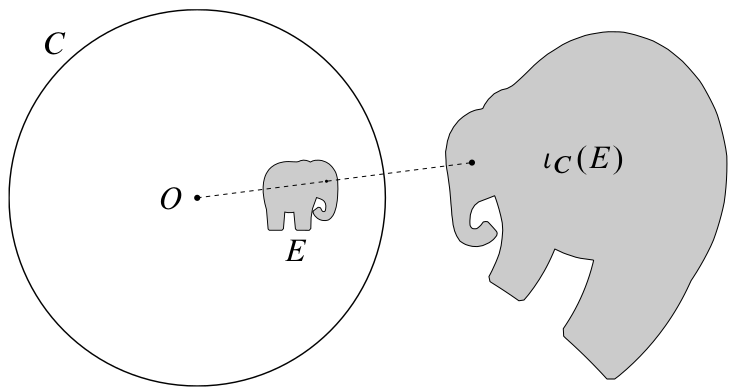
\includegraphics[scale=0.35]{inversao.png}
    \caption{Inversion in $\R^2$}
    \label{fig:5}
\end{figure}

Inversions have the following properties:
\begin{itemize}
    \item $\iota_S$ has order 2, i.e., $\iota_S \circ \iota_S = Id$;
    \item $\iota_S$ fixes any point on C;
    \item $\iota_S$ changes the parts of the plane that are inside and outside C;\\
    $\left(\mbox{Proof: }|OP|<r \Rightarrow |OP*|=\frac{r^2}{|OP|} > r \mbox{ since }|OP|<r\right)$
    \item ($k \leq n$) $\iota_S$ carries k-spheres into k-spheres (remembering that k-planes are k-spheres - they are the ones with $\infty$ radius);
    \item ($k \leq n$) If $S'$ is a k-sphere that contains the center of $S$, then, $\iota_S[S']$ is a k-plane;
    \item $\iota_S$ is a conformal map, i.e., preserves angles between curves;
    \item Considering the isomorphism $\R^2 \cong \C$, if $C$ is the circle of radius 1 and center on $0$, then $\iota_C(z) = \frac{1}{\hat{z}}$ $\left( \mbox{because } z=re^{i\theta}, \frac{1}{\bar{z}} = \frac{1}{re^{-i\theta}} = \frac{e^{i\theta}}{r} = \frac{z}{r^2}\right)$
\end{itemize}

\section{Möbius transformation}\label{TLF} %\cite{Ahlfors}
\subsection{The linear group}

\begin{definicao} The group of linear fractional transformations is defined by
\begin{equation*}
\TLF \doteq \left\{ T:\hat{\C}\rightarrow\hat{\C}\text{; }T(z)=Tz=\frac{az+b}{cz+d}\text{ : }a,b,c,d \in \C\text{; }ad-bc\neq0\text{; }T\infty=\frac{a}{c}\text{; }T(-\frac{d}{c})=\infty \right\}
\end{equation*}
With the composition ($\circ$) operator.\\
T $\in \TLF$ \text{ is called (fractionary) linear transformation or Möbius transformation.}
\end{definicao}

\begin{obs}
It is common to have a $\hat{\C}$ together with $\TLF$, but for technical reasons we will omit it.
\end{obs}

\begin{definicao}
Being
\begin{equation*}
N = \left\{ \alpha I \in \operatorname{M}_{2x2}(\C) : \alpha \in \R^* \right\}
\end{equation*}
The projective special linear group is defined by 
\begin{equation*}
\operatorname{PSL}(2, \C) \doteq \left\{ A = \begin{bmatrix}
a & b\\
c & d
\end{bmatrix} : a,b,c,d \in \C\text{; }det(A)\neq0 \right\} \Bigg/ N
\end{equation*}
with the matrices product operator.
\end{definicao}

\begin{teorema}
We have
\begin{equation*}
(\TLF, \cdot) \cong (\operatorname{PSL}(2, \C), \circ)
\end{equation*}
\text{And the proof is trivial.}
\end{teorema}

Note here that $Tz = \frac{1}{z}$ $\in \TLF$ is a inversion considering the isomorphism $\C \cong \R^2$.

If $c\neq0:$
\begin{gather*}
    \frac{az+b}{cz+d} = \frac{bc-ad}{c^2(z+\frac{d}{c})} + \frac{a}{c}
\end{gather*}
which is a composition of a conjugation, with a translation, an inversion, a rotation, and a homothetic transformation followed by another translation.

If $c=0:$
\begin{gather*}
    \frac{a}{d}z + \frac{b}{d}
\end{gather*}
is a translation followed by rotation and homothetic transformation.

\begin{fato}
\text{Any linear transformation that preserves the real axis can be written with only}\\
\text{real coefficients.}
\end{fato}

%demonstração??

\subsection{Cross ratio} \label{cross}
\begin{definicao}
The cross ratio (z$_1$, z$_2$, z$_3$, z$_4$), with z$_1$, z$_2$, z$_3$, z$_4$ $\in \hat{\C}$ is the image of $z_1$\\
by the linear transformation that carries z$_2$, z$_3$, z$_4$ to 1, 0, $\infty$, in this order.\\
z$_2$, z$_3$, z$_4$ must be distinct because linear transformations are injective.
\end{definicao}

\begin{fato}
Calling S the linear transformation cited above:\\
If z$_2$, z$_3$, z$_4$ $\in \C$:\\
\begin{equation*}
    \operatorname{S}z=\frac{z-z_3}{z-z_4} \cdot \frac{z_2-z_4}{z_2-z_3}
\end{equation*}
If z$_2$, z$_3$ or z$_4$ = $\infty$:\\
\begin{equation*}
    \operatorname{S}z = \frac{z - z_3}{z - z_4} \text{, } \operatorname{S}z = \frac{z_2 - z_4}{z - z_4} \text{, } \operatorname{S}z = \frac{z - z_3}{z_2 - z_3}
\end{equation*}
respectively.
\end{fato}

\begin{fato}
The cross ratio is well defined, i.e., for distinct z$_2$, z$_3$, z$_4$ $\in \hat{\C}$, that is only one linear transformation that carries z$_2$, z$_3$, z$_4$ to 1, 0, $\infty$.
\end{fato}

\begin{proof}
Fix distinct z$_2$, z$_3$, z$_4$ $\in \hat{\C}$ and suppose that S and T $\in$ $\TLF$ carries, respectively z$_2$, z$_3$, z$_4$ to 1, 0, $\infty$.\\
Since ($\TLF$, $\circ$) is a group, $\ST^{-1}$ $\in$ $\TLF$, so that is a, b, c, d $\in \C$ such that
\begin{equation*}
    \ST^{-1}(z) = \frac{az+b}{cz+d}
\end{equation*}
 and since 
 \begin{equation*}
    \ST^{-1}(1) = \frac{a+b}{c+d} = 1;\text{ } \ST^{-1}(0) = \frac{b}{d} = 0;\text{ } \ST^{-1}(\infty) = \frac{a\infty+b}{c\infty+d} = \infty
 \end{equation*}
we have a + b = c + d, b = 0, c = 0, d $\neq \infty$.\\ 
So b = c = 0 and a = d $\neq \infty$, and therefore, $\ST^{-1} = Id$ (identity).
\end{proof}

\begin{teorema}
If T $\in$ $\TLF$, (Tz$_1$, Tz$_2$, Tz$_3$, Tz$_4$) = (z$_1$, z$_2$, z$_3$, z$_4$).
\end{teorema}

\begin{teorema}
(z$_1$, z$_2$, z$_3$, z$_4$) $\in$ $\R$ $\Leftrightarrow$ z$_1$, z$_2$, z$_3$, z$_4$ are in the same circle.
\end{teorema}

\begin{corolario}
Linear transformations carry circles into circles.
\end{corolario}

\begin{fato}
For any z$_2$, z$_3$, z$_4$ $\in$ $\hat{\C}$, distincts, and a$_2$, a$_3$, a$_4$ $\in$ $\hat{\C}$ distincts; there is a linear transformation carrying z$_2$, z$_3$, z$_4$ to a$_2$, a$_3$, a$_4$ in this order.

For that, find the linear transformations that carries z$_2$, z$_3$, z$_4$ into 1, 0, $\infty$ (let's call this one T) and a$_2$, a$_3$, a$_4$ into 1, 0, $\infty$ (this one will be S) and take S$^{-1}$T $\in$ $\TLF$.
\end{fato}

\begin{fato}
In face of the last fact, for any two circles (remembering that lines are circles) that is a linear transformation carrying one to another.

For that, fix 3 points in each circle, apply the last fact and note that for 3 points there is only one circle passing for them and that linear transformations carry circles into circles.
\end{fato}

\subsection{Symmetry}

\begin{definicao}
Let C be a circle on the complex plane, and z$_1$, z$_2$, z$_3$ $\in$ C distincts. The points z, z$^{*}$ $\in \hat{\C}$  are said to be symmetric in relation to C if
\begin{equation*}(z^{*}, z_1, z_2, z_3) = \overline{(z, z_1, z_2, z_3)}.
\end{equation*}
\end{definicao}

\begin{obs}
Fix a circle C; arbitrary distincts points w$_1$, w$_2$, w$_3$ $\in$ C; w, w$^{*}$ $\in$ $\hat{\C}$ and a linear transformation S that carries the real axis into C such that there are distincts a$_1$, a$_2$, a$_3$ $\in \R$ : Sa$_1$=w$_1$, Sa$_2$=w$_2$, Sa$_3$=w$_3$.
\begin{equation*}
    (w^{*}, w_1, w_2, w_3) = \overline{(w, w_1, w_2, w_3)}\Leftrightarrow
\end{equation*}    
%\text{ and since } ($\TLF$, \circ) \text{ is a group, we know that that is }S^{-1} \in $\TLF$, \text{ so we }
\begin{equation*}
    \frac{S^{-1}w^{*}-a_2}{S^{-1}w^{*}-a_3} \cdot \frac{a_1-a_3}{a_1-a_2} = (S^{-1}w^{*}, a_1, a_2, a_3) = \overline{(S^{-1}w, a_1, a_2, a_3)} = \overline{\left(\frac{S^{-1}w-a_2}{S^{-1}w-a_3} \cdot \frac{a_1-a_3}{a_1-a_2}\right)} =
\end{equation*}
\begin{equation*}
    \frac{\overline{S^{-1}w}-a_2}{\overline{S^{-1}w}-a_3} \cdot \frac{a_1-a_3}{a_1-a_2} \Leftrightarrow
\end{equation*}
\begin{equation*}
    \overline{S^{-1}w} = S^{-1}w^{*} \Leftrightarrow    
\end{equation*}
If T is a linear transformation carrying the real axis into C; there are z, z$^{*}$ $\in$ $\hat{\C}$ such that Tz$^*$ = w$^*$ and Tz = w; and $\ST^{-1}$ carries the real axis into itself, then it can be written with only real coefficients, so by the properties of conjugate,
\begin{equation*}
    S^{-1}Tz^{*} = S^{-1}w^{*} = \overline{S^{-1}w} = \overline{S^{-1}Tz} = S^{-1}T\bar{z}
\Leftrightarrow 
\end{equation*}
If T $\in$ $\TLF$ carries the real axis into C and z into w, then carries $\bar{z}$ into w$^{*}$.
\end{obs}

\BlankLine

Directly arrising from that last remark, we have the following properties:
\begin{itemize}
    \item Just the points on C are symmetric to themselves.
    \item The map that carries z to $z^{*}$ is an inversion. [See section \ref{inver}]
    \item Two inversions compposed result in a linear transformation.
\end{itemize}

\begin{teorema} (The symmetry principle)\\
If a linear transformation carries a circle C$_1$ into a circle C$_2$, then it transforms any C$_1$-symmetric pair of points into a C$_2$-symmetric pair.
\end{teorema}

\subsection{Families of circles}
For this study, we will begin fixing a linear transformation:
\begin{gather*}
    \operatorname{T}:\hat{\C} \rightarrow \hat{\C}\\
    \operatorname{T}z = k \frac{z - a}{z - b}
\end{gather*}
$a, b, k$ $\in \C$; $a$ $\neq$ $b$

It is easy to see that a circle that passes through $a$ and $b$ is carried by T to a line that passes through 0 and $\infty$ and that each circle defined by the equation, $\rho \in \R$:

\begin{gather*}
    \frac{|z-a|}{|z-b|} = \frac{\rho}{|k|}
\end{gather*}
will be carried to the circle with center in 0 and radius $\rho$.

Since T $\in$ $\TLF$ is a bijection, the pre-image by T of all the lines that pass through 0 and $\infty$, which union results in the entire plane, is the set of all the circles that pass through $a$ and $b$ (we'll call it C$_1$), with union resulting also in the whole plane. Besides that, the pre-image by T of all the circles centered in 0, that, united with \{ $a, b$ \}, covers the plane completely is the set of all the circles that have fixed ratio of the distance to $a$ by the distance to $b$ (we'll call it C$_2$, and these circles are called Apollonian circles), which also covers the entire plane with the exception of the points $a$ and $b$.

\begin{figure}[H]
    \centering
    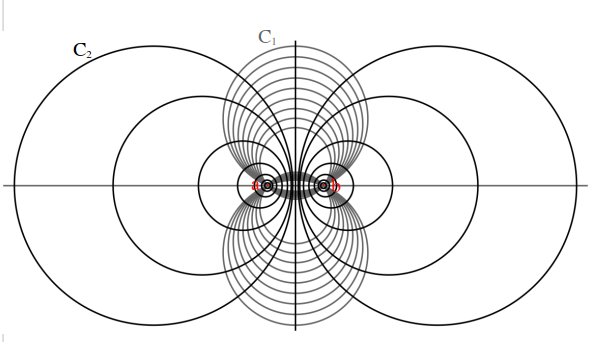
\includegraphics[scale=0.35]{steiner.png}
    \caption{C$_1$ and C$_2$, which together form the denominated circular net or Steiner circles.}
    \label{fig:steiner}
\end{figure}

These families present the following properties:
\begin{itemize}
    \item In the plane, for each point that is not $a$ nor $b$, passes one circle from C$_1$ and another from C$_2$;
    \item $\alpha_1 \perp \alpha_2, \forall \alpha_1 \in$ C$_1,  \alpha_2 \in$ C$_2$;
    \item $\forall \hat{\alpha}_1 \neq \alpha_1 \in$ C$_1$, $\hat{\alpha}_2 \neq \alpha_2 \in $C$_2$,
    \begin{equation*}
    \iota_{\alpha_1}[\alpha_2] = \alpha_2,\text{  } \iota_{\alpha_2}[\alpha_1] = \alpha_1, \text{  } \iota_{\alpha_1}[\hat{\alpha}_1] \in \operatorname{C}_1\setminus{\{\hat{\alpha}_1\}}, \text{  } \iota_{\alpha_2}[\hat{\alpha}_2] \in \operatorname{C}_2\setminus{\{\hat{\alpha}_2\}}
    \end{equation*}
    \item $a$ and $b$ are symmetric only in relation to the circles of C$_2$.
\end{itemize}

\subsubsection{Linear transformations between families of circles}

If T $\in$ $\TLF$ carries $a$ to $a$' and $b$ to $b$', because of [section \ref{cross}], that is $k \in \C$ such that

\begin{gather*}
    \frac{\operatorname{T}z-a'}{\operatorname{T}z-b'} = k \frac{z-a}{z-b}, \forall z \in \hat{\C}
\end{gather*}

It is clear that T carries C$_1$ and C$_2$ respectively into C'$_1$ and C'$_2$, the Steiner circles with foci $a$ and $b$ and $a$' and $b$', in order.

If $a' = a$ and $b' = b$, $a$ and $b$ are called fixed points of T and stay convenient represent z and Tz on the same plane.

Under these circumstances, the whole circular net is mapped into itself.

The value of $k$ serves to identify the image cicles C'$_1$ and C'$_2$. In fact, with appropriate orientation, $\forall \alpha_1 \in$ C$_1$, the angle between $\alpha_1$ and $T[\alpha_1]$ is $arg(k)$, and obviously
\begin{equation*}
    \frac{\frac{|\operatorname{T}z-a|}{|\operatorname{T}z-b|}}{\frac{|z-a|}{|z-b|}} = |k|, \forall z \in \alpha_2, \forall \alpha_2 \in \famcirc_2,
\end{equation*}
i.e., the quocient of the constant ratios of each circle in C$_2$ and their images are given by $k$.

The special cases in which 
\begin{equation*}
    \operatorname{T}[\alpha_1]=\alpha_1, \forall \alpha_1 \in \famcirc_1
\end{equation*}
or
\begin{equation*}
\operatorname{T}[\alpha_2]=\alpha_2, \forall \alpha_2 \in \famcirc_2    
\end{equation*}
are particularly important.

The first case occurs when $k>0$ and the linear transformation will be called hiperbolic. And the other, in which T will be called elliptic, occurs when $|k|=1$.

\begin{proposicao}
Let $\operatorname{g} : S^2 \rightarrow \hat{\C}$ be a stereographic projection [See section \ref{projest}] (considering the isomorphism $\R^2 \cong \C$).\\
Then \\
$R : S^2 \rightarrow S^2$ is a rotation on $S^2$ $\Leftrightarrow \operatorname{g} \circ R \circ \operatorname{g}^{-1}$ is elliptic and has two fixed points: $a$ and $-\frac{1}{a}$, with $a \in \hat{\C}$
\end{proposicao}

\begin{obs}
It means that the image of parallel circles on S$^2$ by stereographic projection will be Apollonian circles on $\R^2 \cong \C$.
[Proof in appendix - proof \ref{proofRemark3}]
\end{obs}

%%%%%%%%%%%%%%%%%%%%%%%%%%%%%%%%%%%%%%%%%%%%%%%%%%%%%%%%%%%%%%%%%%%%%
%    proof 1
%%%%%%%%%%%%%%%%%%%%%%%%%%%%%%%%%%%%%%%%%%%%%%%%%%%%%%%%%%%%%%%%%%%%%

%This project consisted of a detailed study of 3-sphere isomorphisms, an important 3-manifold.

%O projeto consistiu no estudo detalhado de isomorfismos da 3-esfera, uma importante 3-variedade.\hfill \break

\section{Spheres}

Here we start our discussion about the 3-sphere, and for that, we declare now its general definition.

\begin{definicao}[n-sphere]
The n-sphere, $n \in \N$,  S$^n$ is the subset of $\R^n$ with points that have a distance 1 from the origin, i.e.,
\begin{equation*}
    S^{n} = \{x \in \R^{n} : || x || = 1\}
\end{equation*}
\end{definicao}

\section{3-sphere is a 3-manifold}

\begin{definicao}[Topological n-manifold]
A (topological) n-manifold is a Hausdorff topological space M with an enumerable basis such that $\forall$ p $\in$ M there is a neighborhood U of p homeomorphic to an open set in $\R^n$
\end{definicao}

We won't prove it because it is out of our scope, but it is well known that S$^3$ is a Hausdorff topological space with an enumerable basis. The second part of the requirements will be clear by the end of the next section.

\section{3-sphere as one-point compactification of $\R^3$}
S$^3$ is homeomorphic to $\hat{\R}^3$ and this homeomorphism is given by the stereographic projection g, which is an extension of a restriction of an inversion.

\subsection{General case} \label{projest}
In the general case, with $\vec{x} \in \R^{n}$ and $t \in \R$, we have:

\begin{gather*}
\operatorname{g} : S^n \rightarrow \hat{\R}^n \\
\operatorname{g}(\vec{x}, t) =
    \begin{cases}
        \infty, \text{ if }\vec{x} = 0, t = 1 \\
        \frac{1}{1 - t} \vec{x}, \mbox{ } c.c.
    \end{cases}
\end{gather*}

And g is a homeomorphism. [Proof in appendix - proof \ref{proofghomeo}]

%%%%%%%%%%%%%%%%%%%%%%%%%%%%%%%%%%%%%%%%%%%%%%%%%%%%%%%%%%%%%%%%%%%%%%% proof
%%%%%%%%%%%%%%%%%%%%%%%%%%%%%%%%%%%%%%%%%%%%%%%%%%%%%%%%%%%%%%%%%%%%%%

\subsection{Stereographic projection and inversion}

In $\R^{n+1}$, let S be the sphere with center $(0, ..., 0, 1)$ and radius $\sqrt{2}$\\
And let's consider the inversion in $S$, which can be given by the formula:
%(it is easy noting that $\iota_{S}$ is the composition ):

\begin{equation*}
    \iota_{S}(x_1, ..., x_n, t) = \left( \frac{2(x_1, ..., x_n)}{||(x_1, ..., x_n)||^2 + (t-1)^2}, \frac{2(t-1)}{||(x_1, ..., x_n)||^2 + (t-1)^2} + 1 \right)
\end{equation*}

Since S$^n$ contains the center of S, $\iota_s[S^n]$ is a n-plane [See section \ref{inver}].

In fact, we have:

\begin{equation*}
    \forall (x_1, ..., x_n, t) \in S^n \Rightarrow ||(x_1, ..., x_n)||^2+t^2=1
\end{equation*}

\begin{equation*}
    \iota_{S}(x_1, ..., x_n, t) = \left( \frac{2(x_1, ..., x_n)}{||(x_1, ..., x_n)||^2 + (t-1)^2}, \frac{2(t-1)}{||(x_1, ..., x_n)||^2 + (t-1)^2} + 1 \right) =
\end{equation*}

\begin{equation*}
    \left( \frac{(x_1, ..., x_n)}{1-t}, \frac{2t-2}{2-2t}+1 \right) = \left( \frac{(x_1, ..., x_n)}{1-t}, 0 \right)
\end{equation*}

So,

\begin{gather*}
\operatorname{g} : S^n \rightarrow \hat{\R}^n \\
\operatorname{g}(\vec{x}, t) =
    \begin{cases}
        \infty, \text{ if }\vec{x} = 0, t = 1 \\
        \frac{1}{1 - t} \vec{x} \cong \iota_{S}(\vec{x}, t), \mbox{ } c.c.
    \end{cases}
\end{gather*}

%\subsection{2-sphere case}
%
%\begin{equation*}
%g : S^2 \rightarrow \hat{\R}^2 \\
%\end{equation*}
%\begin{align*}
%g(0, 0, 1) = \infty \\
%g(x_1, x_2, t) = \frac{1}{1 - t} \cdot (x_1, x_2) \\
%\end{align*}
%
%Since $\R^2 \cong \C$ and 
%
%\begin{equation*}
%g : S^2 \rightarrow \hat{\R}^2 \\
%\end{equation*}
%\begin{align*}
%g(0, 0, 1) = \infty \\
%g(x_1, x_2, t) = \frac{1}{1 - t} \cdot (x_1, x_2) \\
%\end{align*}
%

\subsection{3-sphere case}

\begin{gather*}
\operatorname{g} : S^3 \rightarrow \hat{\R}^3 \\
\operatorname{g}(x_1, x_2, x_3, t) =
    \begin{cases}
        \infty,\text{ if } x_1 = x_2 = x_3 = 0, t = 1 \\
        \frac{1}{1 - t} (x_1, x_2, x_3), \text{ } c.c.
    \end{cases}
\end{gather*}

With that, g is the homeomorphism between S$^3$ and $\hat{\R}^3$.

Knowing that is a Hausdorff topological space with an enumerable basis, it is clear now that S$^3$ is a 3-manifold.

\subsection{1-sphere case}
The 1-sphere case, however, has an easier approach.

For each point P or Q in the 1-sphere, we can define 
\begin{align*}
    \operatorname{g}(0, 1) = \infty\mbox{, }\operatorname{g}(P) = P^*\mbox{ and }\operatorname{g}(Q) = Q^* 
\end{align*}
as the figure below and find their coordinates using similarity of triangles.

\begin{figure}[H]
    \centering
    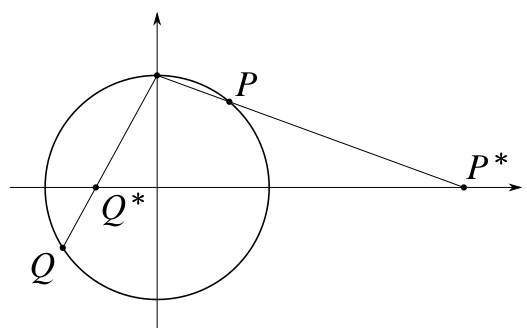
\includegraphics[scale=0.35]{projCirculo.png}
    \caption{Stereographic projection on 1-sphere case}
    \label{fig:projcirc}
\end{figure}

\section{3-sphere as a subset of the quaternions}
In here, we use the well known correspondence $(a,b,c,d) \in \R^4 \leftrightarrow a+bi+cj+dk \in \Hi$, and get:

\begin{equation*}
    S^{3} = \{a + bi+ cj + dk \in \Hi \cong \R^{4} : a^{2} + b^{2} + c^{2} + d^{2} = 1\}
\end{equation*}

\section{3-sphere as a matricial group}
%
%\subsection{1-sphere case}
%
%\begin{teorema}
%$S^{1} \cong SO(2)$
%\end{teorema}
%
%$SO(2) = \{ A \in M_{2x2}(\R) : A^{T}A = I$ and det(A) = 1 \}
%
%\begin{demonstracao}
%Firstly, note that
%\begin{gather*}
%    \psi: S^1 \rightarrow SO(2)\\
%    \psi(a+ib)=M_{a,b}=\begin{bmatrix}
%    a & -b\\
%    b & a
%    \end{bmatrix}
%\end{gather*}
%is a homomorphism.\\
%And since $z=a+ib \in S^1$ such that $\psi(z)=I$ %$\Rightarrow$ $a=1$ and $b=0$ $\Rightarrow z=1$,\\
%we have that $\psi$ is a monomorphism.\\
%
%Let A$=\begin{bmatrix}
%    a_{11} & a_{12}\\
%    a_{21} & a_{22}
%    \end{bmatrix} \in SO(2)$, we want $z$ in $S^1$
%\end{demonstracao}
%
%\subsection{3-sphere case}
%

Firstly, we'll define the special unitary group of degree 2:
\begin{equation*}
 SU(2) \doteq \{ A \in M_{2x2}(\C) : A^{*}A = AA^{*} = I \text{ and }|\det(A)| = 1 \}
\end{equation*}

\begin{teorema}
\begin{equation*}
    S^{3} \cong SU(2)
\end{equation*}
[Proof in appendix - proof \ref{proofTeoSU2}]
\end{teorema}

%%%%%%%%%%%%%%%%%%%%%%%%%%%%%%%%%%%%%%%%%%%%%%%%%%%%%%%%%%%%%%%%%%%%%%% proof
%%%%%%%%%%%%%%%%%%%%%%%%%%%%%%%%%%%%%%%%%%%%%%%%%%%%%%%%%%%%%%%%%%%%%%

\section{3-sphere as a union of circles (1-spheres) - Hopf fibration} %label?

We'll use here the correspondence 

\begin{equation*}
    a+bi+cj+dk \in \Hi \leftrightarrow (a+bi, c+di) \in \C^2.
\end{equation*}

So, $S^3$ can be written as 
\begin{equation*}
    S^3 = \{(a+bi, c+di) \in \C^2 : a^2+b^2+c^2+d^2=1\}
\end{equation*}

And then, we have:

\begin{equation*}
S^3 = \bigcup\limits_{q \in S^3} \{ e^{it}q : t \in \R \}
\end{equation*}
\begin{equation*}
= \bigcup\limits_{q \in S^3} \{ \lambda \cdot q \in \Hi : \lambda \in \C \} \cap S^3
\end{equation*}
\begin{equation*}
\cong \bigcup\limits_{(a+bi, c+di) \in S^3} \{ e^{it}(a+bi, c+di) \in \C^2 : t \in \R \}
\end{equation*}
\begin{equation}\label{direccoord}
     = \bigcup\limits_{(a+bi, c+di) \in S^3} \{ e^{it}(a+bi) \in \C : t \in \R \} \times \{ e^{it}(c+di) \in \C: t \in \R \}
\end{equation}

Note here that $|a+bi|^2 + |c+di|^2 = 1$
\\

The first equality is easy to prove:
\begin{equation*}
    \forall q \in S^3, q \in \{ e^{it}q : t \in \R \} 
\end{equation*}
\begin{equation*}
    \mbox{ and   } \forall t \in \R, \forall q \in S^3, ||e^{it}q||=||e^{it}|| \cdot ||q||=1\cdot1=1
\end{equation*}

The rest of them are trivial.

\begin{equation*}
\phi : \R \times S^3 \rightarrow S^3,
\end{equation*}
\begin{equation*}
\phi(t, q) = e^{it} \cdot q    
\end{equation*}
is a flow named Hopf flow. %pois

\begin{equation*}
\forall q \in S^3, \{ e^{it}q : t \in \R \},    
\end{equation*}
the Hopf flow orbit, is a simple closed curve and for different points in the 3-sphere, those sets are disjoint. %pois

\begin{equation*}
\forall q \in S^3, \{ \lambda \cdot q \in \Hi : \lambda \in \C \}    
\end{equation*}
is a 2-dimensional (real dimension) linear subspace and all points on
\begin{equation*}
\{ e^{it}q : t \in \R \}    
\end{equation*}
have distance 1 from the origin, therefore 
\begin{equation*}
\{ \lambda \cdot q \in \Hi : \lambda \in \C \} \cap S^3    
\end{equation*}
is a great circle in S$^3$.


\section{The 3-sphere as a union of tori}
Having seen the last section, it is easy to declare:

\begin{gather*}
S^3 = \bigcup\limits_{(z,w) \in S^3} \{ e^{it}z \in \C : t \in \R \} \times \{ e^{it}w \in \C: t \in \R \} \mbox{ with } |z|^2 + |w|^2 = 1 \\
= \bigcup\limits_{0 \leq r \leq 1} \bigcup \{\{ e^{it}z \in \C : t \in \R \} \times \{ e^{it}w \in \C: t \in \R \} : |z|^2 = r^2 \mbox{ and } |w|^2 = 1-r^2\} \\
= \bigcup\limits_{0 \leq r \leq 1} \{ z \in \C : |z| = r \} \times \{ w \in \C : |w| = \sqrt{1-r^2} \}. \\
\end{gather*}

\begin{equation*}
 \forall 0 \leq r \leq 1, \{ z \in \C : |z| = r \} \times \{ w \in \C : |w| = \sqrt{1-r^2} \}
\end{equation*}
is called Hopf torus.

If r = 0, 1; the Hopf torus will be a circle - a degenerate torus.
As r increases from 0 to 1, the torus will interpolate those circles, passing from tori much close to the circle of r = 0, to tori close to the one of r = 1.

Here, we can also easily note that for each 0 $<$ r $<$ 1, the Hopf torus is a disjoint union of Hopf circles:

\begin{equation*}
    \{ z \in \C : |z| = r \} \times \{ w \in \C : |w| = \sqrt{1-r^2} \}
\end{equation*}

\begin{equation*}
    = \bigcup\limits_{(a+bi,c+di) \in S^3, |a+bi|=r} \{ e^{it}(a+bi) \in \C : t \in \R \} \times \{ e^{it}(c+di) \in \C: t \in \R \}
\end{equation*}

\section{Those fibrations in $\R^3$}

%Beginning with the Hopf torus, we will prove that each one of them will be sent by the stereographic projection to a ring torus in $\R^3$, being the circle a degenerate torus.

Each Hopf torus will be sent by the stereographic projection to a ring torus in $\R^3$, being the circle a degenerate torus. And those ring tori are all concentric. [Proof in appendix - proof \ref{proofHopfStereo}]

\begin{figure}[H]
    \centering
    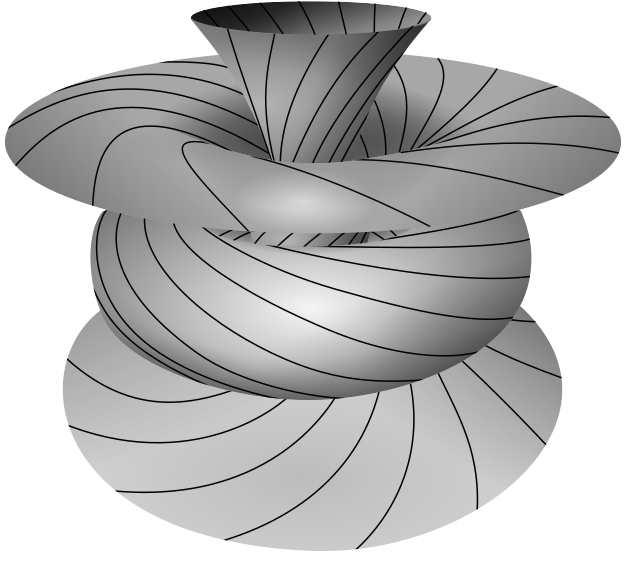
\includegraphics[scale=0.35]{torosHopf.png}
    \caption{The image by a stereographic projection of three non-degenerate Hopf tori (two of them are cut and the image of some Hopf circles is also drawn).}
    \label{fig:3}
\end{figure}

%%%%%%%%%%%%%%%%%%%%%%%%%%%%%%%%%%%%%%%%%%%%%%%%%%%%%%%%%%%%%%%%%%%%%%% proof
%%%%%%%%%%%%%%%%%%%%%%%%%%%%%%%%%%%%%%%%%%%%%%%%%%%%%%%%%%%%%%%%%%%%%%

Now about each Hopf circle, on equation \ref{direccoord}, one can note that any Hopf circle takes a turn in each of the coordinated directions of the Hopf torus in which it is. Consequently, the same will occur with their images by stereographic projection, remembering that every ring torus is homeomorphic to the cartesian product of two circles. Then, each Hopf circle will be sent to a Villarceau circle.

\begin{figure}[H]
    \centering
    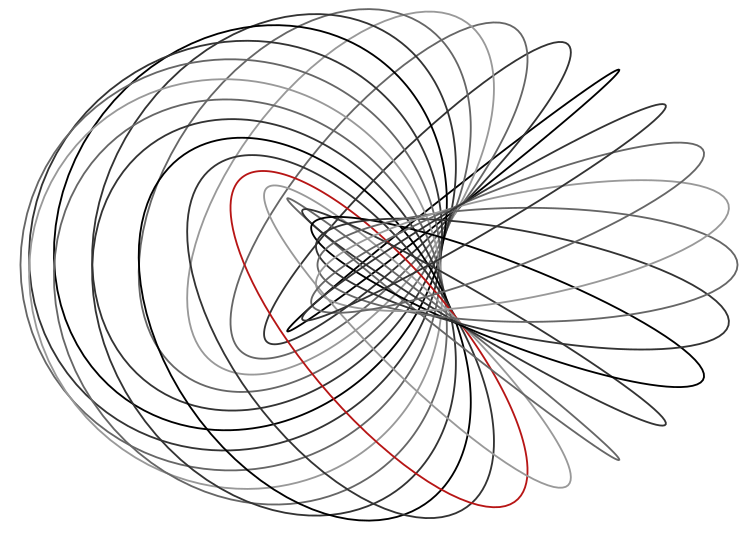
\includegraphics[scale=0.35]{toroHopf.png}
    \caption{Stereographic projection of some Hopf circles in the same Hopf torus.}
    \label{fig:toroHopf}
\end{figure}

\section{Villarceau circles}

Villarceau circles are the ones that "take a turn in each of the circles of the cartesian product form of the torus".\\
We'll show here that they exist and how they are.\\
Given a torus, if they exist, being circles, they would be 2 real dimensional, and since thay take a turn in each of the circles of the cartesian product form of the torus, would be given by the section of a torus along a diagonal plane bitangent that passes through the center of the torus. Taking this intersection, if it give us circles, will be the Villarceau circles. So let's put a coordinate system and prove that:\\

\begin{figure}[H]
    \centering
    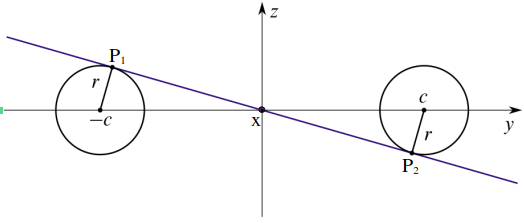
\includegraphics[scale=0.35]{villar.png}
    \caption{The central vertical section of the union of the plane and torus described above with the coordinates chosen. Imagine the hole figure with the torus being given by the rotation of these two circles around the z-axis and with the plane being the one that have the x-axis and the purple line.}
    \label{fig:villar}
\end{figure}

Equation of the torus:

\begin{gather*}
    (x^2+y^2+c^2-r^2)^2 = 4c^2(x^2+y^2)
\end{gather*}

Equation of the plane:

\begin{gather*}
    \sqrt{c^2-r^2}z+ry=0
\end{gather*}

So, the intersection of these figures will be given by the solution set A of:

\begin{gather*}
    \begin{cases}
        (x^2+y^2+c^2-r^2)^2 = 4c^2(x^2+y^2)\\
        \sqrt{c^2-r^2}z+ry=0
    \end{cases}
\end{gather*}

But since

\begin{gather*}
    (x^2+y^2+c^2-r^2)^2 = 4c^2(x^2+y^2) \Leftrightarrow (x^2+y^2+r^2-c^2)^2 - 4r^2x^2 = 4r^2y^2 - 4(c^2-r^2)z^2
\end{gather*}

We have:

\begin{gather*}
    \begin{cases}
        (x^2+y^2+c^2-r^2)^2 = 4c^2(x^2+y^2)\\
        \sqrt{c^2-r^2}z+ry=0
    \end{cases}
    \Leftrightarrow
    \begin{cases}
        \sqrt{c^2-r^2}z+ry=0\\
        (x^2+y^2+r^2-c^2)^2 - 4r^2x^2 = 4r^2y^2 - 4(c^2-r^2)z^2 = 0
    \end{cases}\\
    \Leftrightarrow
    \begin{cases}
        \sqrt{c^2-r^2}z+ry=0\\
        (x^2+y^+z^2+r^2-c^2+2rx)(x^2+y^2+z^2+r^2-c^2-2rx) = 0
    \end{cases}
    \Leftrightarrow\\
    \begin{cases}
        \sqrt{c^2-r^2}z+ry=0\\
        ((x+r)^2+y^2+z^2-c^2)((x-r)^2+y^2+z^2-c^2) = 0
    \end{cases}
\end{gather*}

And then, $A = A_1 \cup A_2$, being
\begin{gather*}
    A_1 \text{ the solution set of } \alpha_1 = 
    \begin{cases}
        \sqrt{c^2-r^2}z+ry=0\\
        (x+r)^2+y^2+z^2-c^2 = 0 \text{ (*)}
    \end{cases}\\
    \text{and } A_2 \text{ the solution set of } \alpha_2 = 
    \begin{cases}
        \sqrt{c^2-r^2}z+ry=0\\
        (x-r)^2+y^2+z^2-c^2 = 0 \text{ (**)}
    \end{cases}
\end{gather*}

Since (*) and (**) are equations of different 2-spheres and $P_1$ and $P_2$ are different points that are in $A_1$ and $A_2$ (the non-empty intersection of a sphere with a plane is either a single point, or a circle), we have that A is the union of two circles $A_1$ and $A_2$, both with radius $c$ and enteirely on the initial plane, but $A_1$ with center $(-r, 0, 0)$ and $A_2$ centered on $(r, 0, 0)$, the just proved Villarceau circles in this imposed coordinate system.
%\section{3-sphere as two solid tori}
%
%\begin{figure}[H]
%    \centering
%    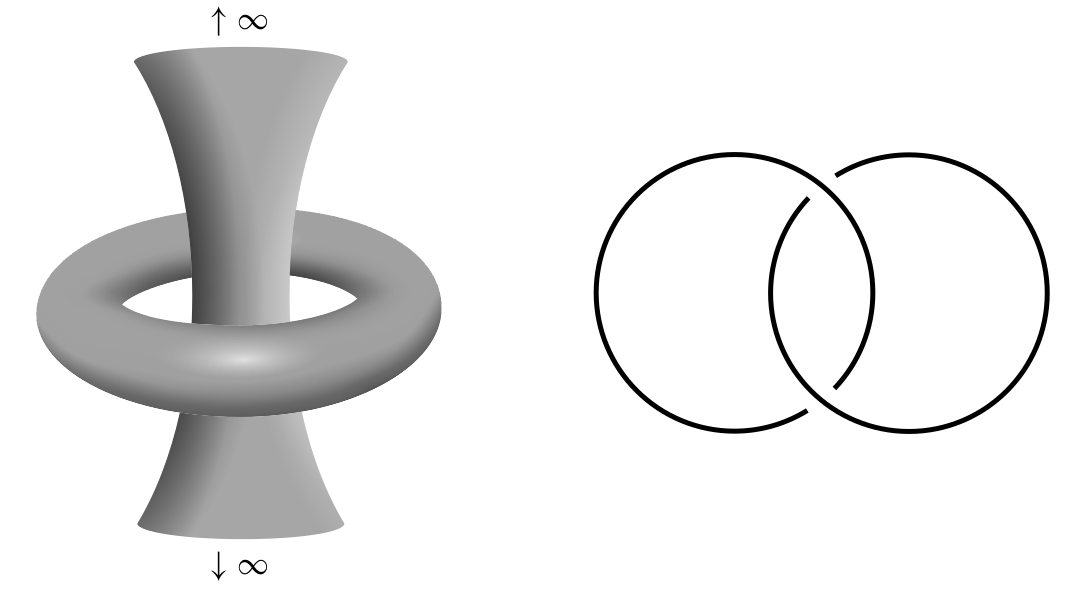
\includegraphics[scale=0.35]{torosSolid.png}
%    \caption{}
%    \label{fig:0}
%\end{figure}
%
%\section{3-sphere as a Lie group}
%
%SU(2) $\cong$ S$^3$ is an example of a Lie group, a group, which we know that SU(2) is, that is also a smooth manifold, which we know that S$^3$ is.
%
%The related Lie algebra will be \textswab{SU}(2) = $\{ ui + vj + wk \in \Hi : u, v, w \in \R\}$.